\chapter{Analysis of high-temperature events}

\label{Chapter5}

In this chapter, the products of HTE monitoring from MITIP will presented firstly using several scenes worldwide which contains volcanoes, large scale lava flow and wild fires. In section 5.2, the HTE monitoring results of MITIP will be compared with the results of the Zhukov's algorithm, which is used to process the TET-1 imagery in the receive center.\\
%----------------------------------------------------------------------------------------
%	SECTION 1
%----------------------------------------------------------------------------------------

\section{High-temperature events}
In this section, the HTE monitoring results are presented. For the processing of all scenes, the maps of MODIS water vapor, ASTER DEM and 8.6 $\mu$m emissivity were provided and resampled to the TET-1 imagery's size and pixel size. The input TET-1 MIR and TIR TOA radiance values are scaled with scale factor 1.15 and 1.05 respectively.\\

%-----------------------------------
%	SUBSECTION 1
%-----------------------------------

\subsection{Volcanoes}
First of all, the HTE monitoring products of Etna and Stromboli in the date 2016.06.22 are presented. Both of them only occupy a little spaces in images because of their small sizes.

\begin{figure}[!htbp]
\centering
\subfigure[MIR band]{
\label{fig:Etna_mir_tem}
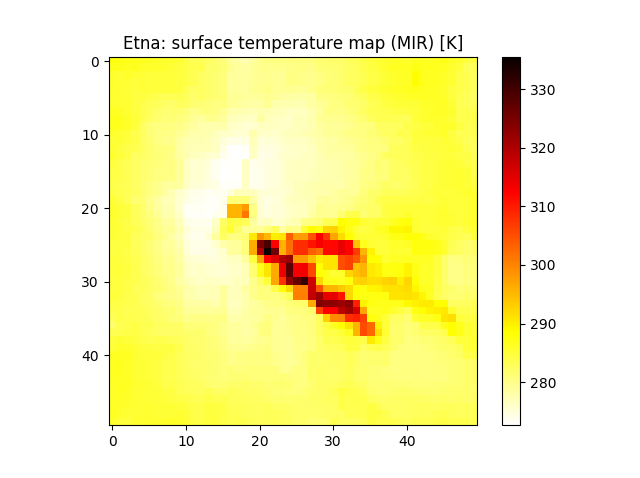
\includegraphics[width = 0.8\linewidth]{temp_map_etna_mir.png}}
\hspace{0.1in}
\subfigure[TIR band]{
\label{fig:Etna_tir_tem}
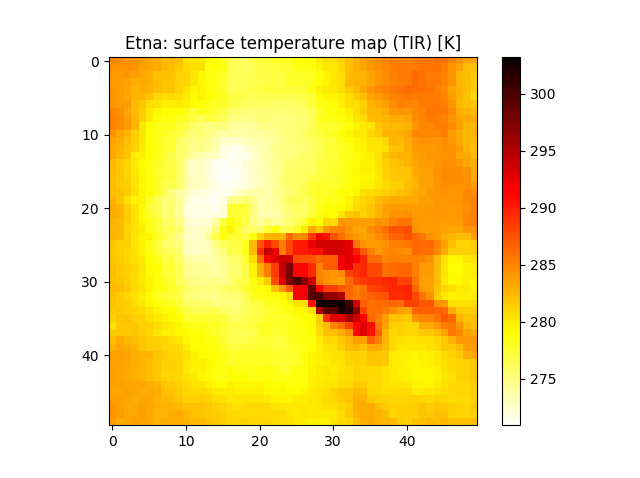
\includegraphics[width = 0.8\linewidth]{temp_map_etna_tir.png}}
\caption{Surface temperature maps of Etna 2014.06.22.}
\label{fig:Etna_sur_tem}
\end{figure}

\noindent As Figure \ref{fig:Etna_sur_tem} shows, the surface temperatures of the lava are around 310 K to 340K in MIR band and 290K to 310K in TIR band. The effective target temperature in sub-pixel resolution and effective target pixel fraction as well as the FRP are shown in Figure \ref{fig:Etna_HTE} and Figure \ref{fig:Etna_frp}. We can see that no all hot pixels in the surface temperature maps are solved for the effective target temperature and target pixel fraction due to numerical reasons. The hottest areas of the Etna is around 850 K. It can be notice that the higher the effective target temperature in one pixel, the lower the effective target pixel fraction of it. Because the pixel temperature and background temperature are pre-determined.\\

\begin{figure}[!htbp]
\centering
\subfigure[Effective target temperature]{
\label{fig:Etna_eff_tem}
\includegraphics[width = 0.8\linewidth]{Effective_target_tem_etna.png}}
\hspace{0.1in}
\subfigure[Effective target pixel fraction]{
\label{fig:Etna_eff_fra}
\includegraphics[width = 0.8\linewidth]{Effective_target_pixel_frac_etna.png}}
\caption{HTE monitoring products of Etna 2014.06.22.}
\label{fig:Etna_HTE}
\end{figure}

\begin{figure}[!htbp]
\centering
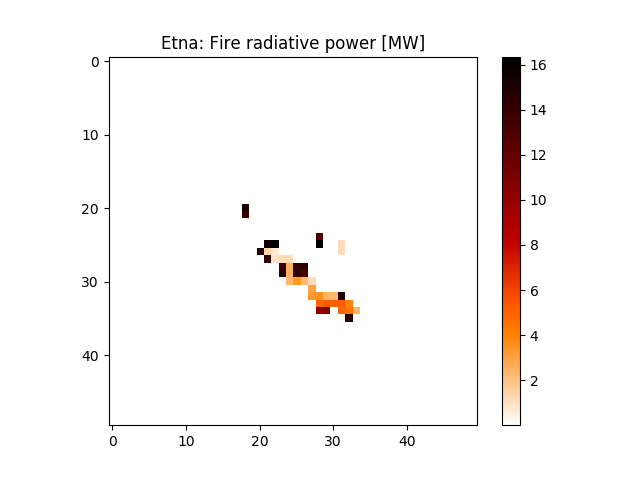
\includegraphics[width=0.8\linewidth]{frp_etna.png}
\caption{FRP of Etna 2014.06.22.}
\label{fig:Etna_frp}
\end{figure}

\noindent Stromboli island is one of the Aeolian island of Italy. The Stromboli volcano is one of the most active volcanoes on Earth. It has been nearly continuous eruption for about 2000 years. Since there is a small town in Stromboli island, the prediction and monitoring of the eruption of the Stromboli volcano is of great importance. The figure \ref{fig:Strom_sur_tem} shows the surface temperature maps of Stromboli in MIR and TIR band respectively of the date 2014.06.22. It can be notice that in Summer's evening, the temperature of the sea surface is higher than the temperature of the land surface.\\

\begin{figure}
\centering
\subfigure[MIR band]{
\label{fig:Strom_mir_tem}
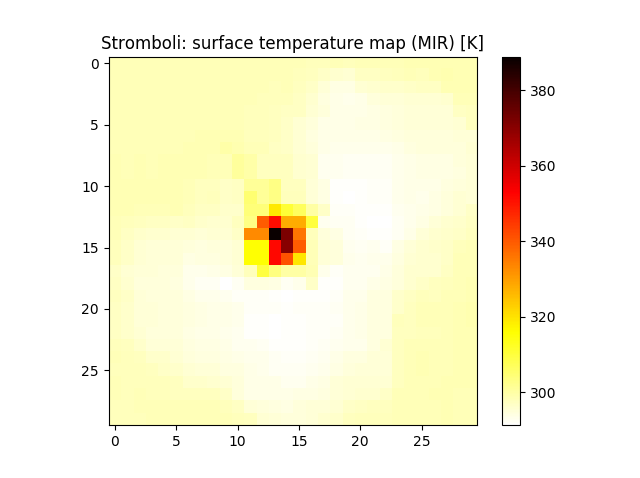
\includegraphics[width = 0.8\linewidth]{strom_tem_mir.png}}
\hspace{0.1in}
\subfigure[TIR band]{
\label{fig:Strom_tir_tem}
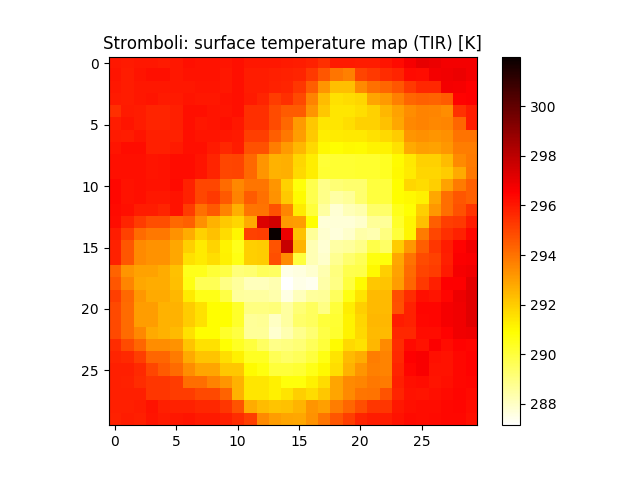
\includegraphics[width = 0.8\linewidth]{strom_tem_tir.png}}
\caption{Surface temperature maps of Stromboli 2014.06.22.}
\label{fig:Strom_sur_tem}
\end{figure}

\noindent The effective target temperature and effective target pixel fraction of Stromboli in date 2014.06.22 are shown in Figure \ref{fig:Strom_HTE} and the fire radiative power in Figure \ref{fig:Strom_frp}. We can see that the hottest areas of the Stromboli is above 1400 K which only occupy a small fraction of the pixels as well.\\

\begin{figure}[!htbp]
\centering
\subfigure[Effective target temperature]{
\label{fig:Strom_eff_tem}
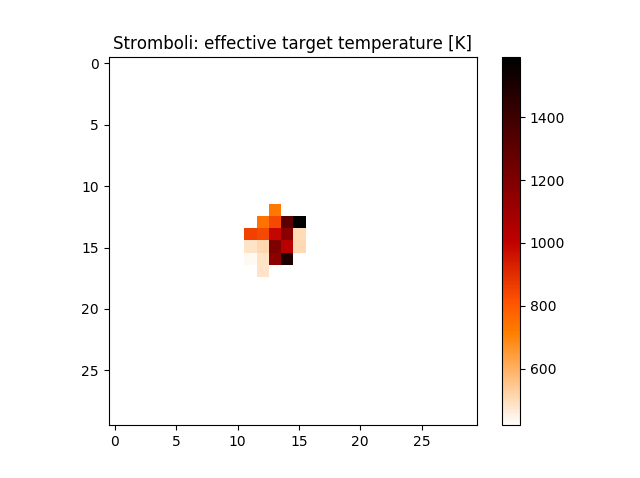
\includegraphics[width = 0.8\linewidth]{strom_eff_tem_strom.png}}
\hspace{0.1in}
\subfigure[Effective target pixel fraction]{
\label{fig:Strom_eff_fra}
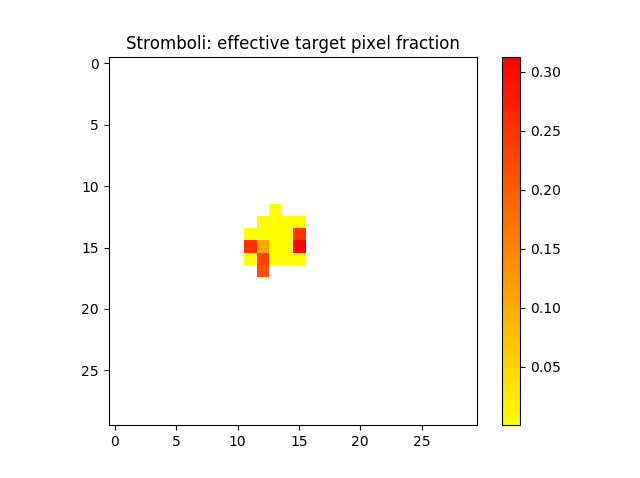
\includegraphics[width = 0.8\linewidth]{strom_eff_pixel_frac_strom.png}}
\caption{HTE monitoring products of Stromboli 2014.06.22.}
\label{fig:Strom_HTE}
\end{figure}

\begin{figure}[!htbp]
\centering
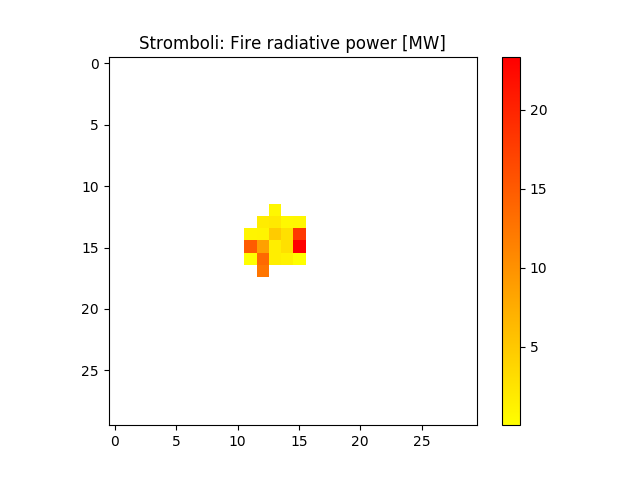
\includegraphics[width=0.8\linewidth]{frp_strom.png}
\caption{FRP of Stromboli 2014.06.22.}
\label{fig:Strom_frp}
\end{figure}

\noindent Etna and Stromboli are both small volcanoes which only occupy around 20 pixels in the imageries. In contrast, the eruption of Bardarbunga is much more intensive and its lava occupies a much larger area. Bardarbunga is a subglacial stratovolcano located in Iceland. The last eruption of Bardarbunga is from August 2014 to February 2015. Figure \ref{fig:Bar_sur_tem} presents the surface temperature map of Bardarbunga in date 2014.09.24.\\

\begin{figure}
\centering
\subfigure[MIR band]{
\label{fig:Bar_mir_tem}
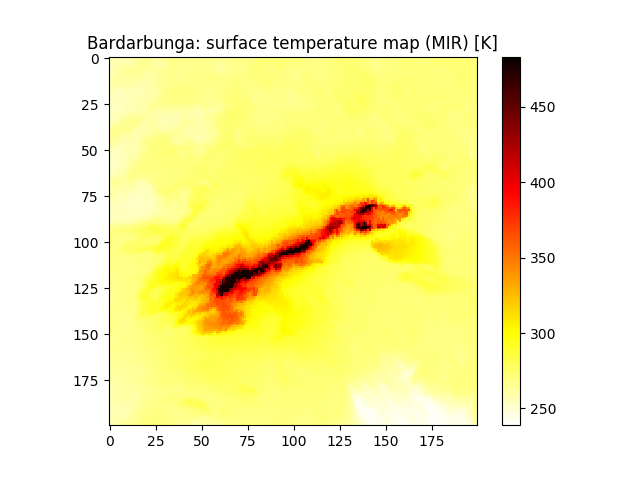
\includegraphics[width = 0.8\linewidth]{Bar_tem_mir.png}}
\hspace{0.1in}
\subfigure[TIR band]{
\label{fig:Bar_tir_tem}
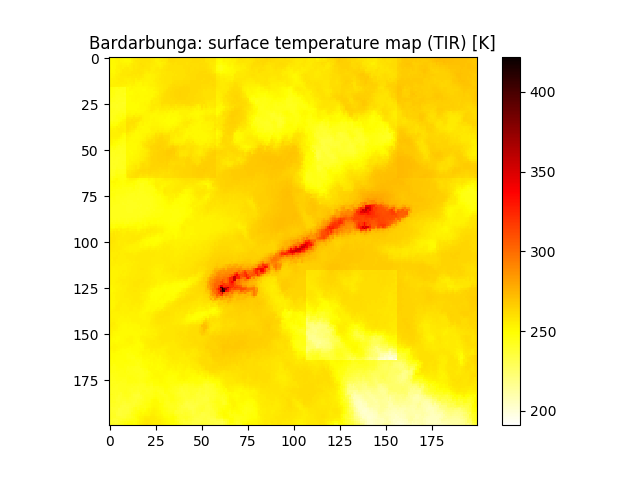
\includegraphics[width = 0.8\linewidth]{Bar_tem_tir.png}}
\caption{Surface temperature maps of Bardarbunga 2014.09.14.}
\label{fig:Bar_sur_tem}
\end{figure}

\noindent It is clear to see that the erupted lava occupied a large area and the temperature of it is between 400 K and 500 K in MIR band and 350 K to 450 K in TIR band. Figure \ref{fig:Bar_HTE} and Figure \ref{fig:Bar_frp} give the effective target temperature and effective target pixel fraction as well as FRP maps.\

\begin{figure}[!htbp]
\centering
\subfigure[Effective target temperature]{
\label{fig:Bar_eff_tem}
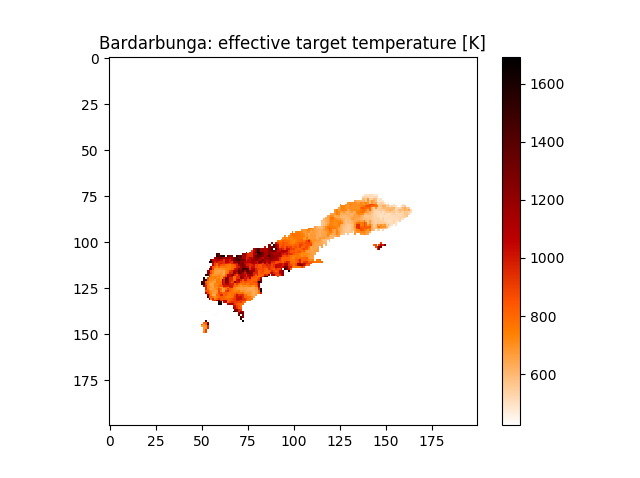
\includegraphics[width = 0.8\linewidth]{Bar_eff_tem.png}}
\hspace{0.1in}
\subfigure[Effective target pixel fraction]{
\label{fig:Bar_eff_fra}
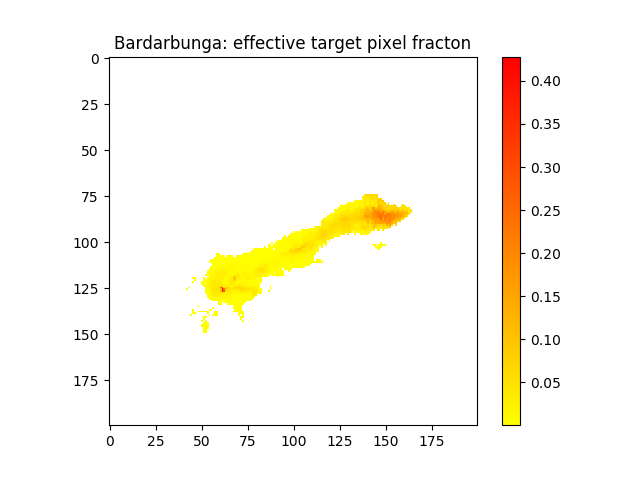
\includegraphics[width = 0.8\linewidth]{Bar_eff_pixel_frac.png}}
\caption{HTE monitoring products of Bardarbunga 2014.09.14.}
\label{fig:Bar_HTE}
\end{figure}

\begin{figure}[!htbp]
\centering
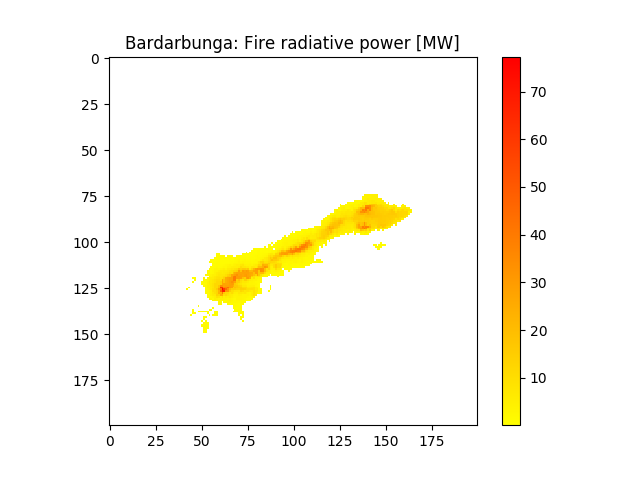
\includegraphics[width=0.8\linewidth]{Bar_frp.png}
\caption{FRP of Bardarbunga 2014.09.14.}
\label{fig:Bar_frp}
\end{figure}
%-----------------------------------
%	SUBSECTION 2
%-----------------------------------

\subsection{Fire events}
Besides volcanoes, wild fires are another kind of high-temperature events need to be paid attention to. Here, the HTE monitoring results of Portugal wild fires will be presented. Figure \ref{fig:Por_sur_tem} shows the surface temperature maps in MIR and TIR band. The fire edges can be seen clearly in the surface temperature maps.\\

\begin{figure}
\centering
\subfigure[MIR band]{
\label{fig:Por_mir_tem}
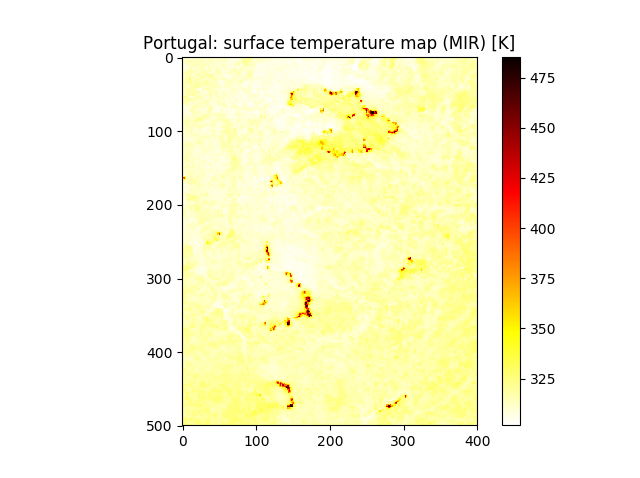
\includegraphics[width = 0.8\linewidth]{Por_tem_mir.png}}
\hspace{0.1in}
\subfigure[TIR band]{
\label{fig:Por_tir_tem}
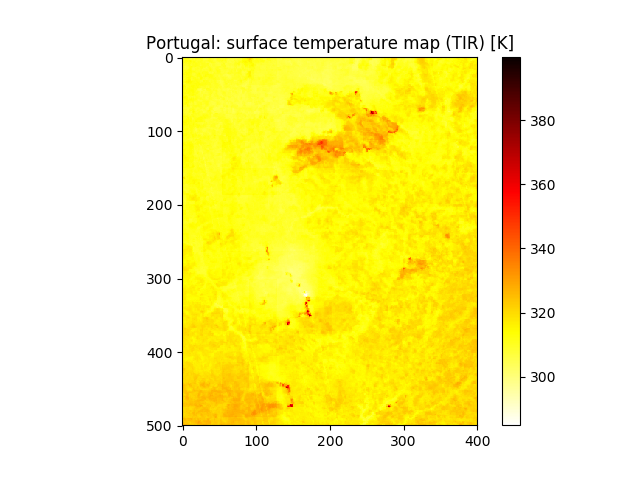
\includegraphics[width = 0.8\linewidth]{Por_tem_tir.png}}
\caption{Surface temperature maps of Portugal wild fires in 2016.08.11.}
\label{fig:Por_sur_tem}
\end{figure}

\noindent Figure \ref{fig:Por_HTE} and Figure \ref{fig:Por_frp} are the effective target temperature and effective target pixel fraction as well as fire radiative power maps. We can see the large scale and the scorching temperatures of the wild fires.

\begin{figure}[!htbp]
\centering
\subfigure[Effective target temperature]{
\label{fig:Por_eff_tem}
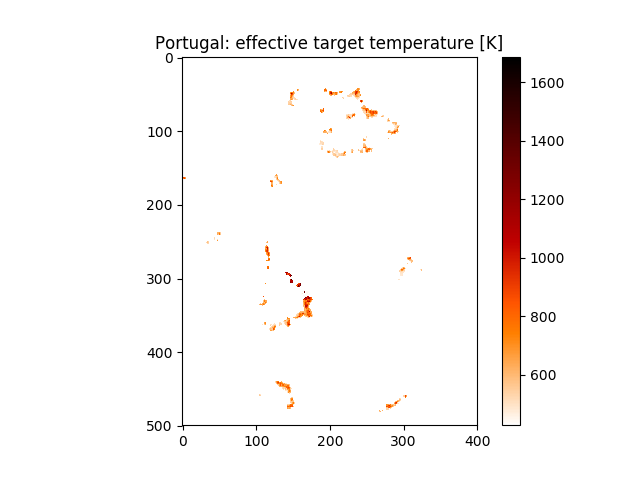
\includegraphics[width = 0.8\linewidth]{Por_eff_tem.png}}
\hspace{0.1in}
\subfigure[Effective target pixel fraction]{
\label{fig:Por_eff_fra}
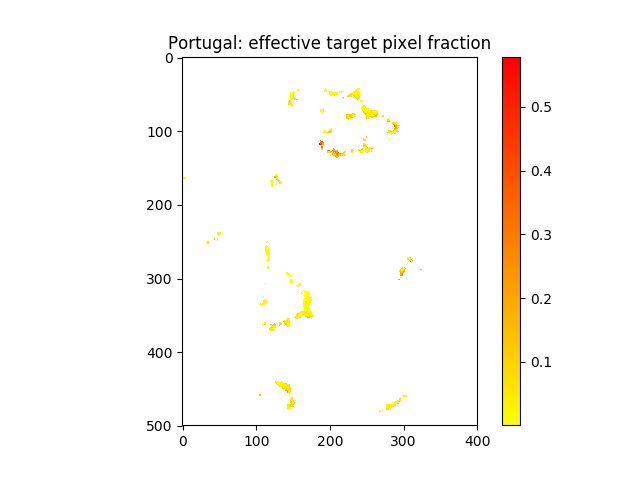
\includegraphics[width = 0.8\linewidth]{Por_eff_pixel_frac.png}}
\caption{HTE monitoring products of Portugal wild fires in 2016.08.11.}
\label{fig:Por_HTE}
\end{figure}

\begin{figure}[!htbp]
\centering
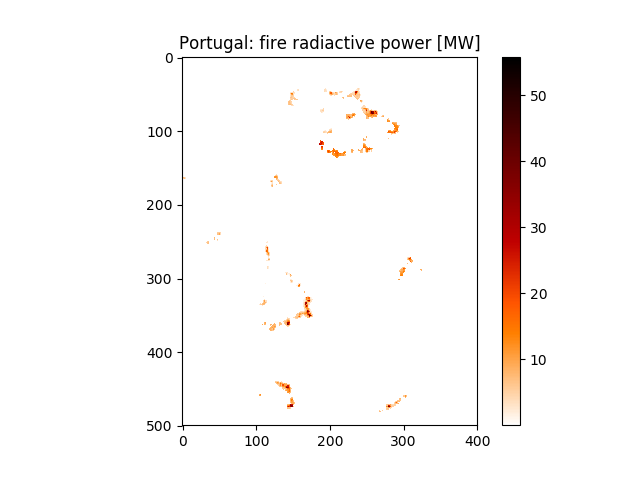
\includegraphics[width=0.8\linewidth]{Por_frp.png}
\caption{FRP of Portugal wild fires in 2016.08.11.}
\label{fig:Por_frp}
\end{figure}

%----------------------------------------------------------------------------------------
%	SECTION 2
%----------------------------------------------------------------------------------------

\section{Comparison with the results of the Zhukov's algorithm}
In this section, the HTE monitoring products of MITIP are compared with the results of Zhukov's algorithm, which used to process the TET-1 imagery originally.\\

\noindent The Zhukov's algorithm carries out a bundle of tests to filter out clouds, warm soils and fire scars etc first and then performs fire pixel detection and quantification. It uses the dual channel method stated in Chapter 2 to determine temperature in sub-pixel resolution as well. However, the Zhukov's algorithm detects and quantifies the hot area by means of per cluster instead of per pixel as MITIP method dose. After detection, the Zhukov's algorithm aggregates hot pixels which are neighbors to form a hot cluster and the temperature of this cluster and its area etc are estimated.\\

\noindent But the MITIP method performs a pixel-based analysis. Consequently, in order to compare the results of them, a procedure is developed to shift the MITIP's original pixel-based results to a cluster-based results. The input is the effective target temperature map, which is converted to vector file afterwards. Then each polygon features in this vector file is extracted and converted to a mask file. The mask file is used to extract AOI in the effective target temperature map and doing zonal statistics of the AOI. The final output is the cluster's temperature and size.\\


%-----------------------------------
%	SUBSECTION 1
%-----------------------------------

\subsection{Brief description of Zhukov's algorithm}

%-----------------------------------
%	SUBSECTION 2
%-----------------------------------

\subsection{From pixel-based to cluster-based analysis}

%-----------------------------------
%	SUBSECTION 3
%-----------------------------------

\subsection{Comparision}

%----------------------------------------------------------------------------------------
%	SECTION 3
%----------------------------------------------------------------------------------------

% \section{Bardarbunga}

%----------------------------------------------------------------------------------------
%	SECTION 4
%----------------------------------------------------------------------------------------

% \section{Chile}

%----------------------------------------------------------------------------------------
%	SECTION 5
%----------------------------------------------------------------------------------------

% \section{Portugal}